\documentclass[frenchb]{article}
\usepackage[T1]{fontenc}
\usepackage[latin1]{inputenc}
%Pour utilisation sous unix
%\usepackage[utf8]{inputenc}
%\usepackage[utf8x]{inputenc}
\usepackage{a4wide}
\usepackage{graphicx}
\usepackage{amssymb}
\usepackage{color}
\usepackage{babel}

\begin{document}

\begin{figure}[t]
\centering

\includegraphics[width=5cm]{inp_n7.png}
\end{figure}

\title{\vspace{4cm} \textbf{Projet:Codage de Huffman}}
\author{MANUEL D'UTILISATION}
\date{\vspace{7cm} Departement Sciences du Numerique - Premiere annee \\
2021-2022 }

\maketitle

\newpage
\section{Compresser}
\Large Pour utiliser notre programme de compression sur un fichier texte de votre choix il faudra suivre la syntaxe suivante :\\\\

\begin{figure}[ht!]
    				\centering
                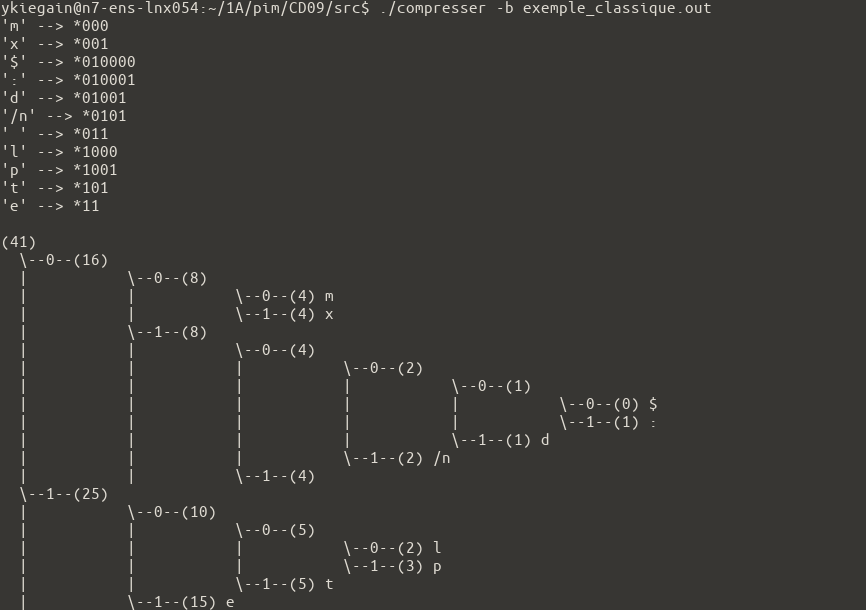
\includegraphics[scale=0.4]{tableabrhuffman.png} 
				\end{figure}

\textbf{./compresser [-OPTIONS] NOMDUFICHIER}\\
OPTIONS : b | bavard :  permet de generer l'affichage de l'arbre d'Huffman qui aura ete utilise pour la compression du fichier texte, ainsi que la table d'huffman donnant pour chaque caractere son codage d'Huffman dans l'arbre. \\\\
Cette commande produit un fichier nomme :\\ \textbf{NOMDUFICHIER\_compresse.hff} qui contient une succesion d'octet permettant de retrouver le fichier texte initiale grace a la commande de decompression\\

A noter que en cas de lancement du programme avec des parametres incorrect, la bonne syntaxe d'utilisation de celui-ci vous sera rappeler dans le flux de sortie en vigueur.
  \

\section{Decompresser}
Pour utiliser la commande de decompression quand a elle, il faudra suivre la syntaxe suivante : \\\\ \textbf{./decompresser NOMDUFICHIER}\\\\
Cette commande est fournie sans option elle generera juste dans le repertoire courant, le fichier texte dont le fichier compresse est issue
sous le nom : \textbf{NOMDUFICHIER\_decompresse.out}\\

A noter que en cas de lancement du programme avec des parametres incorrect, la bonne syntaxe d'utilisation de celui-ci vous sera rappeler dans le flux de sortie en vigueur.
	

\end{document} 